\section{Rayonnement dipolaire électrique}

Le rayonnement électromagnétique est un phénomène fondamental. Toute charge en mouvement accéléré rayonne un champ [$\vec{E},\vec{B}$] et donc de l'énergie électromagnétique.

\subsection{Le modèle du dipôle électrique oscillant}

On a une distribution neutre, et on fait l'hypothèse que les charges mobiles sont en mouvement sinusoïdal. Par exemple, un atome possède une charge $q>0$ fixe (le noyau) et une charge $-q<0$ mobile (électrons). On peut donc le modéliser avec un dipôle comme à la Figure~\ref{fig:modelisation_atome_dipole_oscillant}. Dans ce cas, le mouvement est~$z(t)=z_{0}\cos(\omega t)$, et le moment dipolaire est
\begin{equation*}
    \boxed{
        \vec{p}(t)=q\vec{G^{-}O}(t)=-qz_{0}\cos(\omega t)\vec{u_{z}}.
    }
\end{equation*}

\begin{figure}
    \centering
    \tikzsetnextfilename{modelisation_atome_dipole_oscillant}
    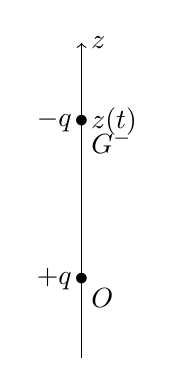
\begin{tikzpicture}[scale=1]  
        % \helpgrid{3}{3}
        \draw[->] (0,0)--++(0,4) node [right] {$z$};
        \node at (0,3) {$\bullet$};
        \node at (0,3) [left] {$-q$};
        \node at (0,3) [right] {$z(t)$};
        \node at (0,3) [below right] {$G^{-}$};
        \node at (0,1) {$\bullet$};
        \node at (0,1) [left] {$+q$};
        \node at (0,1) [below right] {$O$};
    \end{tikzpicture}
    \caption{Modélisation d'un atome par un dipôle électrique oscillant.}    
    \label{fig:modelisation_atome_dipole_oscillant}
\end{figure}

En ordre de grandeur, on a $p_{0}\sim 10^{-29}\si{\coulomb\metre}$.